% Klassifiziert den Dokumenten-Typ
% Doku: http://exp1.fkp.physik.tu-darmstadt.de/tuddesign/
% Farben: http://www.tu-darmstadt.de/media/medien_stabsstelle_km/services/medien_cd/das_bild_der_tu_darmstadt.pdf
%  bigchapter: Chapter haben doppelte Schriftgröße
%  linedtoc: Linien im Inhaltsverzeichnis wie bei Überschriften
%  colorbacktitle: Der Dokumenten-Titel wird mir der Accentfarbe hinterlegt
\documentclass[bigchapter,colorback,accentcolor=tud4b,linedtoc,11pt]{tudreport}

% Input Dokument hat das Encoding UTF-8
\usepackage[utf8]{inputenc}
% Wichtiges Paket für Links und verlinktes Inhaltsverzeichnis
\usepackage[ngerman]{hyperref}
% Paket für Fußnoten
\usepackage[stable]{footmisc}
% Paket für amsmath (aligned mathe formeln)
\usepackage{amsmath}
% Paket für Bibliotheks-Verzeichnis, square: Verwende eckige statt runde klammern
% \usepackage[square]{natbib}
% Paket zum Plotten von Datensätzen
\usepackage{pgfplots}
\pgfkeys{%
  /pgfplots/Streudaten/.style={%
    /pgf/number format/use comma,
    legend pos=north east,
    xlabel=Streuvektor s in 1/nm,
    x tick label style={/pgf/number format/1000 sep=},
    ylabel=$I\cdot s^{2}$,
    y tick label style={/pgf/number format/1000 sep=},
    width=0.38\linewidth,
    height=0.40\linewidth,
    scale only axis,
    xmin=0,
    xmax=0.44,
    grid=both,
    ymin=-10,
    %ymax=0.0045,
    tick align=outside,
    tickpos=left,
    minor x tick num=3,
    minor y tick num=4,
    minor grid style={dotted,thin}
  }
}

\pgfkeys{%
  /pgfplots/Autokorrel/.style={%
    /pgf/number format/use comma,
    legend pos=north east,
    xlabel=u  in  nm,
    x tick label style={/pgf/number format/1000 sep=},
    ylabel=$K(u)$ in $\frac{e}{nm^{6}}$,
    y tick label style={/pgf/number format/1000 sep=},
    width=0.38\linewidth,
    height=0.30\linewidth,
    scale only axis,
    xmin=0,
    xmax=25,
    grid=both,
    ymin=-105,
    ymax=155,
    tick align=outside,
    tickpos=left,
    minor x tick num=3,
    minor y tick num=4,
    minor grid style={dotted,thin}
  }
}

\pgfkeys{%
  /pgfplots/tabh/.style={%
    /pgf/number format/use comma,
    legend pos=north east,
    x tick label style={/pgf/number format/1000 sep=},
    xlabel=Unterkühlung in $K$,
    y tick label style={/pgf/number format/1000 sep=},
    width=0.38\linewidth,
    height=0.30\linewidth,
    scale only axis,
    xmin=0,
    xmax=100,
    grid=both,
    ymin=3,
    ymax=6,
    tick align=outside,
    tickpos=left,
    minor x tick num=3,
    minor y tick num=4,
    minor grid style={dotted,thin}
  }
}

% Anhänge für Original-Messdaten
\usepackage{fancyvrb}

% redefine \VerbatimInput
\RecustomVerbatimCommand{\VerbatimInput}{VerbatimInput}%
{fontsize=\footnotesize,
 %
 frame=lines,  % top and bottom rule only
 framesep=2em, % separation between frame and text
 fontsize=\scriptsize,
 %
 labelposition=topline,
 %
 commandchars=\|\(\), % escape character and argument delimiters for
                      % commands within the verbatim
 commentchar=*        % comment character
}

% Polar Plots
\usetikzlibrary{pgfplots.polar}
% Verwende deutsche Bezeichner für Inhaltsverzeichnis, ... (ngerman = New German: neue Rechtschreibung)
\usepackage{ngerman}
% Deutsche Zahlen (entfernt z.B. das Leerzeichen nach einem Dezimal-Komma)
\usepackage{ziffer} 

\usepackage[verbose]{placeins}

%wegen Grafikverschiebung hinzugefügt
\usepackage{float}

%\usepackage{graphicx}
%\usepackage{caption}
\usepackage{subcaption} %Für subfigures

% PDF-Optionen
\hypersetup{%
  pdftitle={TU Darmstadt \- Physikalisches Praktikum für Fortgeschrittene},
  pdfauthor={Esra Bauer und Sören Link},
  pdfsubject={Versuch 1.1},
  pdfview=FitH,
}
% Nummeriere formeln in Subsections einzeln
% Kleines makro zur assymetrischen Fehlerangabe

% Entspricht-Zeichen
\usepackage{scalerel}

\newcommand\equalhat{%
\let\savearraystretch\arraystretch
\renewcommand\arraystretch{0.3}
\begin{array}{c}
\stretchto{
    \scalerel*[\widthof{=}]{\wedge}
    {\rule{1ex}{3ex}}%
}{0.5ex}\\ 
=%
\end{array}
\let\arraystretch\savearraystretch
}
%BEGINN TITELSEITE

\title{Magnetfeldmessung}

\subtitle{Esra Bauer  \\Sören Link}

\subsubtitle{Betreuer: Thore Bahlo \hfill Versuchsdatum: 28. Januar 2015}

\author{Esra Bauer, Sören Link}

%\settitlepicture{img/title.jpg}

\institution{Physikalisches Praktikum \\für Fortgeschrittene \\ Versuch 1.1}

\date{\today}


%ENDE TITELSEITE

\begin{document}
%ANFANG DOKUMENT

%Titelseite einfügen
\maketitle

%Inhaltsverzeichnis einfügen
\tableofcontents

%ANFANG INHALT

\chapter{Einleitung}

In diesem Versuch geht es um die Vermessung von Elektromagneten, wie sie in Teilchenbeschleunigeranlagen eingesetzt werden. In diesem Gebiet ist oft eine hohe Genaugkeit für die Fokussierung und Richtung des Teilchenstrahls erforderlich, weshalb die Magnete präzise gefertigt und montiert werden müssen. Anhand  des Praktikumsversuchs wird aufgezeigt, wie man die charakteristischen Größen der jeweiligen Magnete, also die magnetische Flussdichte eines Dipolmagneten und den Feldgradienten eines Quadrupolmagneten quantitativ untersuchen kann und somit z.B. Rückschlüsse auf die Qualität des Magneten oder dessen Ausrichtung treffen kann.

\chapter{Grundlagen}
\section{Elektromagnetismus}


\subsection{Funktionsweise}

TODO: Ferromagnetismus, Hysterese

\subsection{Bauformen}

TODO: Dipol- Quadrupolmagneten, Multipole

\section{Bewegung geladener Teilchen im Magnetfeld}

TODO: Hall-Effekt, Induktion

\section{Diskrete Fourier-Transformation}


\chapter{Durchführung}
\section{Vermessung des Gradientenprofils des Quadrupols}

Zerst muss überprüft werden, ob die Achsen des Quadrupols und der zum Messen benutzten CNC-Einheit parallel zueinander sind. Dazu wird eine Messung entlang der X-Achse der CNC-Einheit aufgenmmen, welche parallel zur s-Achse einen potentiell durch den Quadrupol geführten Teilchenstrahl liegen sollte. Bei korrekter Positioneirung des Quadrupols ist zwischen dem steilen Anstieg bzw.\ Abfall an den Rändern des Quadrupols ein bereich konstanter Magnetfeldstärke zu erwarten.
\begin{figure}[H]
\centering
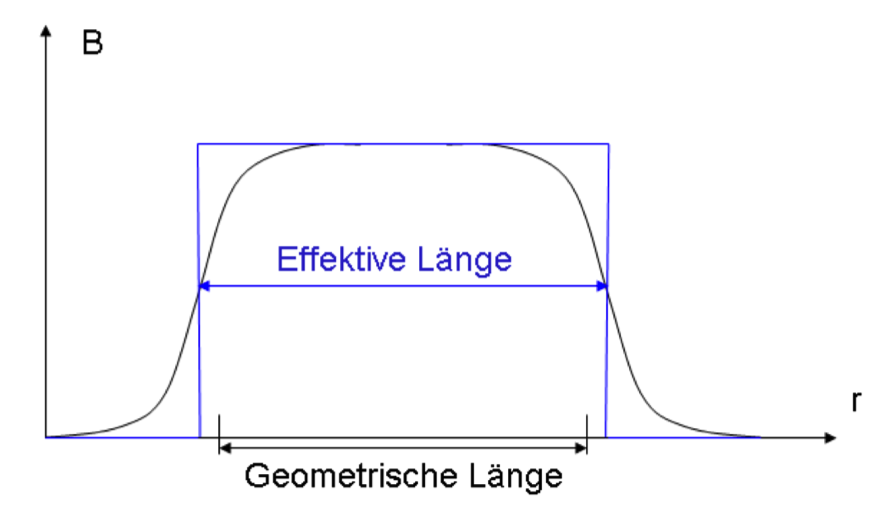
\includegraphics[width=130mm]{img/magnetfeldplateau.png}
\caption{Erwarter Verlauf des gemessenen Magnetfeldes bei korrekter Ausrichtung des Quadrupols \cite{anleitung}}
\end{figure}
In unserem fall war der Quadrupol bereits sehr gut ausgerichtet, im Plateau-Bereich im Inneren des Quadrupols hat sich die Magnetfeldstärke über eine Distanz von etwa $5 cm$ um weniger als $1\%$ verändert. Die Masse und unhandlichen Ausmaße des verwendete Magneten ließen es als sehr unwahrscheinlich erscheinen, duch eine manuelle Korrektur der Ausrichtung des Quadrupols eine Verbesserung zu erzielen, weswegen wir keine veränderungen an der Ausruchtung des Magneten durchgeführt haben.

\begin{center}
\begin{figure}[H]
\begin{tikzpicture}
\begin{axis}[
    legend pos=north west,
    title={Kalibrationsmessung des Quadrupols},
    xlabel=$x$ in $mm$,
    ylabel=$B$ in $mT$,
    width=0.9\textwidth,
    height=7cm,
    xmin=0,
    xmax=225,
    grid=both,
    ymin=0,
    ymax=112,
    tick align=outside,
    tickpos=left,
    minor x tick num=3,
    minor y tick num=4,
    minor grid style={dotted,thin},
]
\addplot[red, smooth, mark=x, mark size=1pt, error bars/.cd, x dir=both, x fixed=0.25]
table[x expr=\thisrowno{0} * 5, y expr=\thisrowno{2} * (-1)] {data/Ausrichtung.txt};
\end{axis}
\end{tikzpicture}
\captionof{figure}{Gemessenes Magnetfeld für die Kalibrationsmessung in Abhängigkeit der Position der Hallsonde entlang der s- bzw.\ x-Achse im Quadrupol. Die Nahezu konstante Feldstärke im Plateaubereich spricht für eine beinahe exakte Ausrichtung des Quadrupols.}
\end{figure}
\end{center}


Zur Vermessung des Quadrupols wird die Magnetfeldstärke im zuerst bei $0 A$ betriebenen Magneten mit einer Hall-Sonde an 45 Messpunkte in $5 mm$ Abständen entlang der X-Achse der CNC-Einheit aufgenommen, wobei soch sowohl die ersten als auch die letzten 6 Messpunkte außerhalb des Quadrupols befinden. Diese Messreihe wird anschließend für 5 weitere Positionen im Quadrupol in Abständen von $8mm$ entlang der Y-Achse der CNC-Einheit widerholt. Diese Messreihe aus insgesamt 270 Messpunkten wurde von einem Computerprogramm nach Eingabe der gewünschten Parameter automatisch durchgeführt.

Im Anschluss wird die Messung für 5 weitere Stromstärken in Schritten von 2A von 10A bis 2A widerholt.

\section{Vermessung des Dipols in der xy-Ebene}
Analog zur Vermessung des Quadrupols wird der der "`Steerer"' Dipol vermessen. Entlang der S-Achse des Magneten bzw.\ der x-Achse der CNC-Einheit werden bei $5 A$ Betriebsstrom 51 Messpunkte im Abstand von $1 cm$ aufgenommen. Diese Messreihe wird für 11 veschiedene Positionen entlang der y-Achse mit einem Abstand von $2 mm$ automatisiert durchgeführt.

Im Gegensatz zum Quadrupol besitzt der Dipol keine abschirmende Eisenplatte an den offenen Enden des Magneten, wodurch das vom Dipol erzeugte Magnetfeld außerhalb der geometrischen Länge des Magneten deutlich langsamer abfällt. Aus diesem Grund werden jeweils 10 Magnetfeldmessungen (entsprechen $10 cm$) außerhalb des Magneten durchgeführt.

\section{Magnetfeld des Dipols in Abhängigkeit des Spulenstroms}

Um den Effekt der Hysterese auf den verwendeten Dipolmagneten zu bestimmen, wird an einer festen Position im Dipol bei Stromstärken in 1A-Schritten von 5A bis 0A die Magnetfeldstärke gemessen. Bei dieser Messung ist besonders darauf zu Achten, die Stromstärke monoton auf den nächsten Messwert herunter zu regeln, da sonst durch die Eigenschaften der Hysterese die Messung verfälscht werden würde.

\section{Messung der Multipolanteile mit rotierender Spule}
Die Vermessung des Multipolanteils im Quadrupol wird mit einer rotierenden Spule im Zentrum des Magneten durchgeführt. Allerdings ergibt sich bei einer solchen Messung das Problem, dass sich durch die Symmetrie des Quadrupols in einer um das Zentrum des Magneten rotierenden Spule alle induzierten Ströme aufheben. Aus diesem Grund wurde die Messspule außermittig an die rotierende Achse des Messgerätes angebracht, was bei korrekter Ausrichtung im Quadrupol zu einer kreisförmigen Rotation der Messpule um den Mittelpol des Magneten führt.

Die zentrale Positionierung der Rotationsachse der Spule erwieß sich dabei als kein triviales Unterfangen, da wir keine Möglichkeit hatten, das innere des Quadrupols und die Position der Sonde genau zu vermessen


\chapter{Auswertung}

\section{Vermessung des Gradientenprofils des Quadrupols}


\section{Vermessung des Dipols in der xy-Ebene}

Fester strom, alle positionen

\section{Magnetfeld des Dipols in Abhängigkeit des Spulenstroms}


\section{Messung der Multipolanteile mit rotierender Spule}

\section{Messung am Oszi zur DFT}

\chapter{Fazit}


%ENDE INHALT
\cleardoublepage{}
% Eintrag fürs Inhaltsverzeichnis
\newpage
\begin{thebibliography}{100}
  \bibitem{anleitung} \url{Versuchsanleitung}
\end{thebibliography}
\end{document}
